% The Gaussian Case
\section{The M-ROC Surface  under Gaussian Hypotheses}
In the following we present two examples, for computing the M-ROC for Gaussian Hypotheses. 

\noindent \textbf{Example 1:}

Assume three hypotheses given as:
\begin{equation}
\label{equ: Gaussian Hypothesis}
\begin{split}
	H_0:\;\;\;\;\;\;\;\;&X \sim \mathcal{N}(-1,1)\\
    H_1:\;\;\;\;\;\;\;\;&X \sim \mathcal{N}(0,1)\\
    H_2:\;\;\;\;\;\;\;\;&X \sim \mathcal{N}(1,10)\,,
\end{split}
\end{equation}
where $\mathcal{N}(\mu,\sigma^2)$ denotes a Gaussian PDF with mean $\mu$ and variance $\sigma^2$.
To form the M-ROC surface, we first consider points that belong to $M_0$.
From section 3.1, we can see that when $(P_d, c_1, c_2) \in M_0$, there exists non-negative $\mathbf{k}$ such that by using decision rule 
\begin{equation}
f_0(x) \substack{H_0 \\ \geq \\ < \\ \bar{H}_0} k_1f_1(x) + k_2f_2(x)
\end{equation}
we have 
\begin{equation}
\begin{split}
\label{1125c0}
&P_d = \int_{-\infty}^{\infty} u(f_0(x) - \sum_{j=1}^{2}k_jf_j(x)) f_0(x)\mathrm{d}x    \,, \\
&P_{f_i} = \int_{-\infty}^{\infty} u(f_0(x) - \sum_{j=1}^{2}k_jf_j(x)) f_i(x) \mathrm{d}x = c_i\;\;\;\;\;    i=1, 2\,.
\end{split}
\end{equation}
We use Matlab to compute the M-ROC for region $M_0$. The values of $k_1$ and $k_2$ range from $0$ to $100$ in steps of $0.01$. Substituting the value of $k_1$ and $k_2$ into \eqref{1125c0}, results in the corresponding $P_d$ $P_{f_1}$ and $P_{f_2}$.  The set $M_0$ is illustrated in Figure \ref{pic: surface for m0 gaussian}, and Figure \ref{pic: contour for m0 gaussian} presents the projection of Figure \ref{pic: surface for m0 gaussian} on the $c_1, c_2$ plane.

\begin{figure}[!t]
\centering
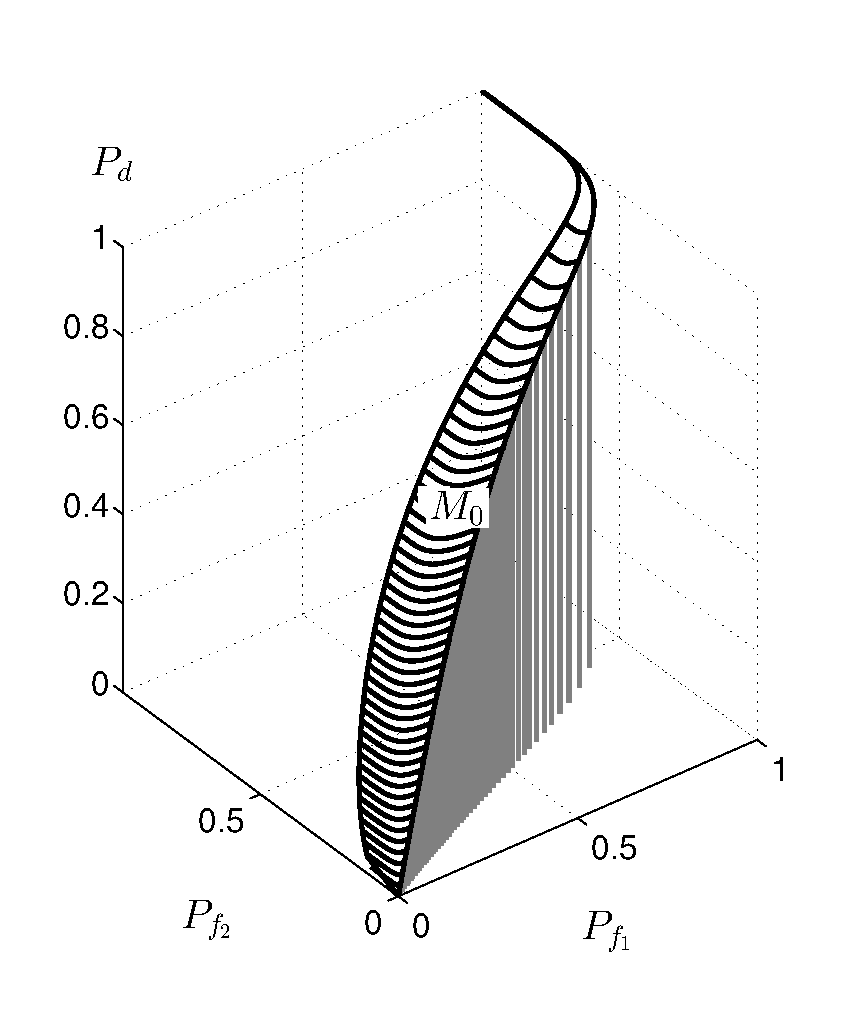
\includegraphics[width=12cm, height=16cm]{3/singleROC.eps}
\caption{Region that can be achieved by Neyman Pearson testing with $k_i \geq 0 (i=1, ..., M)$.}
\label{pic: surface for m0 gaussian}
\end{figure}
\newpage

\begin{figure}[!t]
\centering
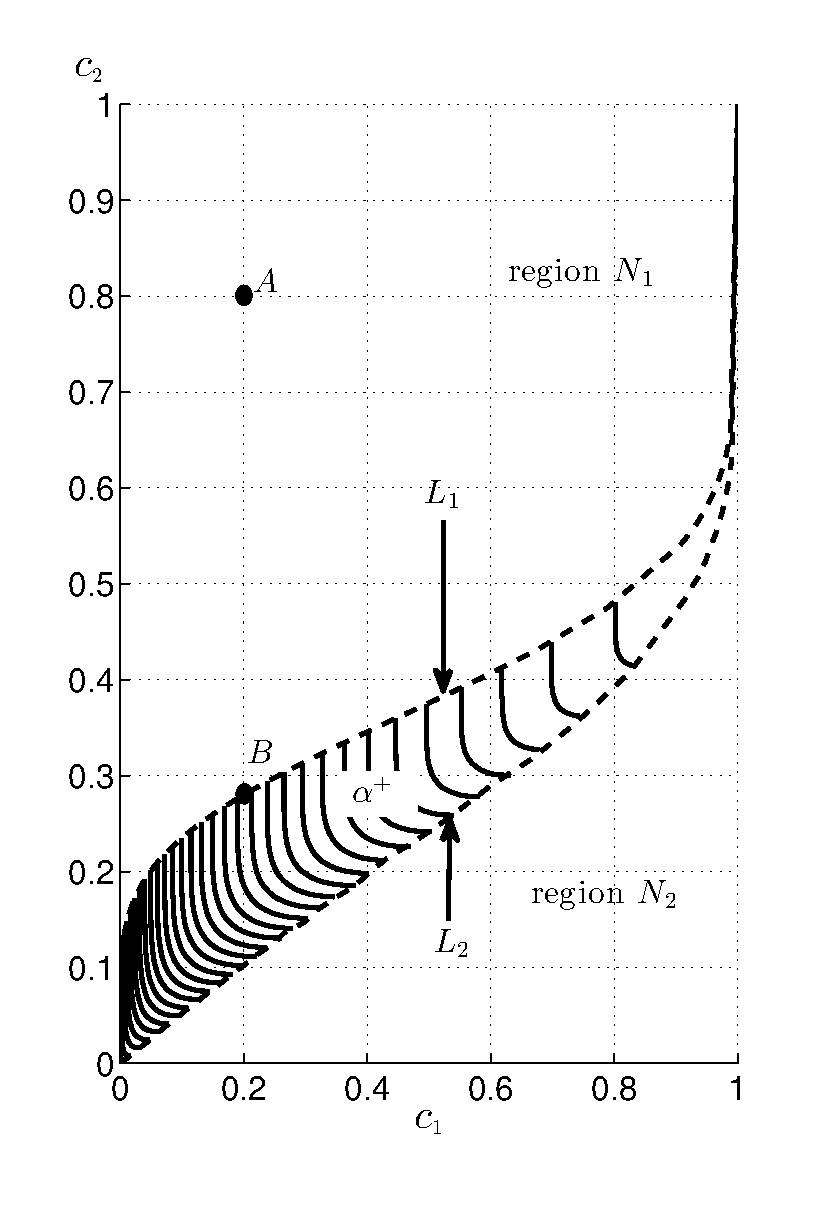
\includegraphics[width=12cm, height = 16cm]{3/singlecontour.eps}
\caption{Region that can be achieved by Neyman Pearson testing with $k_i \geq 0 (i=1, ..., M)$.}
\label{pic: contour for m0 gaussian}
\end{figure}

\begin{figure}[!t]
\centering
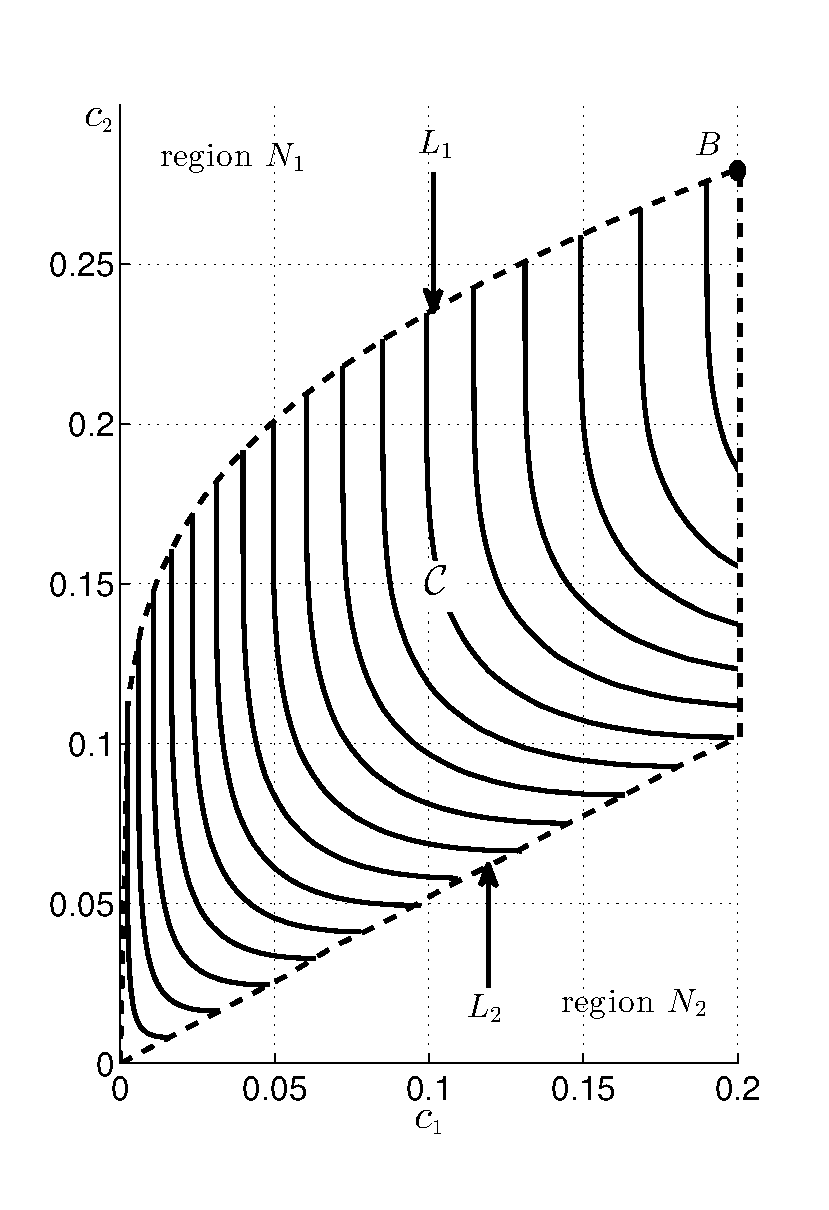
\includegraphics[width=12cm, height = 16cm]{3/singlecontour2.eps}
\caption{The region $\mathcal{C}$ when $c_1 = 0.2$ and $c_2 = 0.8$.}
\label{pic: region C}
\end{figure}

In Figure \ref{pic: contour for m0 gaussian} $N_0$ is the projection of $M_0$ on the $c_1, c_2$ plane. Since $M_0$ is the set of points with $[c_1, c_2] \in \alpha^+$, $N_0$ is the set of points belonging to $\alpha^+$.
Define curve $L_1$ as the set of points 
\[
\{ (c_1, c_2) \in L_1 | (c_1, c_2) \in {N}_0 \;\;\text{and} \;\;(c_1, c_2+\epsilon)\notin {N}_0 \;\;\;\;\text{for any positive $\epsilon$} \}\,.
\]
Define curve $L_2$ as the set of points 

\[
\{ (c_1, c_2) \in L_2 | (c_1, c_2) \in {N}_0 \;\;\text{and} \;\;(c_1 + \epsilon, c_2)\notin {N}_0 \;\;\;\;\text{for any positive $\epsilon$} \}\,.
\]
Let $N_1$ denote the region enclosed by line $c_1 = 0$, $c_2$; line $c_1$, $c_2 = 1$ and curve $L_1$.
Let $N_2$ denote the region enclosed by line $c_1 = 1$, $c_2$; line $c_1$, $c_2 = 0$ and curve $L_2$.
The regions $N_0$ $N_1$ and $N_2$ are shown in Figure \ref{pic: contour for m0 gaussian}.

In the following, we present the decision rule for points belong to regions $N_1$ and $N_2$.

\noindent \textbf{Property 2:}
\textit{\\(1) All points belonging to region $N_1$ or curve $L_1$, if they have the same $c_1$, they have the same decision rule and same $P_d$.
\\(2) All points belonging to region $N_2$ or curve $L_2$, if they have the same $c_2$, they have the same decision rule and same $P_d$.
}

\noindent \textbf{PROOF}
Recall $F(\mathbf{c})$ is defined as the largest $P_d$ that can be achieved under constraint $\mathbf{P}_f = \mathbf{c}$ and 
       $G(\mathbf{c})$ is defined as the largest $P_d$ can be achieved under constraint $\mathbf{P}_f \leq \mathbf{c}$.
Firstly we will show $F(\mathbf{c}) = G(\mathbf{c}) $ when $\mathbf{c} \in \alpha^+$.

According to the definition of $\alpha^+$, for a point $(c_1^0, c_2^0) \in \alpha^+$, there exists a decision rule 
\[
\delta:\;\;\;\;f_0(x) \substack{H_0 \\ \geq \\ < \\ \bar{H}_0} k_1f_1(x) + k_2f_2(x) \;\;\;\;(k_1, k_2 \geq 0)
\]
such that under decision rule $\delta$, we have 
\begin{equation}
\label{1125a3}
\mathbf{P}_{f}(\delta) = \mathbf{c}\,.
\end{equation}
From \textbf{ENP Lemma (\rmnum{2})}, we know 
\begin{equation}
\label{1125c1}
P_d(\delta) = F(\mathbf{c})\,.
\end{equation}
Since $k_1, k_2 \geq 0$, according to \textbf{ENP Lemma (\rmnum{3})}, $\delta$ also achieve the largest $P_d$ while keeping $\mathbf{P_f} \leq \mathbf{c}$, i.e. 
\begin{equation}
 P_d(\delta) =G(\mathbf{c}) 
\label{1125a2}
\end{equation}
From \eqref{1125c1} and \eqref{1125a2} we can see $F(\mathbf{c}) = G(\mathbf{c})$ for $\mathbf{c} \in \alpha^+$.
In the proof of \textbf{Lemma 1} in Chapter 2 Section 2.2,  we have shown $G(\mathbf{c})$ is a non-decreasing function for each variable of $\mathbf{c}$, it can be concluded that $F(\mathbf{c})$ is a non-decreasing function for each variable of $\mathbf{c}$ on set $\alpha^+$.

Now consider point A in region ${N}_1$ with coordinates $(c_1, c_2) = (c_{1_A}, c_{2_A})$. As it is shown in \ref{pic: contour for m0 gaussian}, the decision rule for point A can be computed through MENP (\rmnum{2}). To do it,  we need to determine the set $\mathcal{C}$, which is the intersection of $\mathcal{A}_c$ and $\alpha^+$.  In this case, set $\mathcal{C}$ is plotted in Fig. \ref{pif: regionC}.
According to MENP (\rmnum{2}), we need to find $\mathbf{c}^0 \in \mathcal{C}$ such that it maximum $F(\mathbf{c})$ among all $\mathbf{c} \in \mathcal{C}$.
Figure \ref{pic: contour for m0 gaussian} and Figure \ref{pic: regionC} shows that point B (with coordinate $(c_{1_B}, c_{2_B})$ where $c_{1_B} = c_{1_A}$) has the largest $c_1$ $c_2$ components among all $\mathbf{c} \in \mathcal{C}$. Since $F(\mathbf{c})$ is a non-decreasing function for $c_1$ and $c_2$ on set $\alpha^+$, it can be concluded that for a $\mathbf{c} \in \mathcal{C}$, we have $F(c_{1_B, c_{2_B}}) \geq F(\mathbf{c})$. As point B is in set $\mathcal{C}$, there exists an ENP decision rule with non-negative parameters $\delta^\ast$ such that $P_{f_1}(\delta^\ast) = c_1$ and  $P_{f_2}(\delta^\ast) = c_2$. From MENP (\rmnum{2}), we can conclude $\delta^\ast$ is the optimal decision rule for point A. Thus we can see the optimal decision rule for point A and point B are the same. Since point A lies in region $N_1$, point B lies in region $L_1$ and $c_{1_A} = c_{1_B}$, we can conclude for two points respectively belong to $N_1$ and $L_1$, if they have the same $c_1$ component, they have the same decision rule and same $P_d$. 

Furthermore, we can see as long as A is in region $N_1$ its decision rule only depends on the value of $c_{1}$.  In other words, as long as A is still in region $N_1$, with $c_1 = c_{1_A}$ fixed,  when $c_{2}$ changes, the decision rule and $P_d$ remain the same. Hence we can conclude all points belonging to region $N_1$ or curve $L_1$, if they have the same $c_1$, they have the same decision rule and same $P_d$.

In the same way, we can prove: For points belong to region $N_2$ or curve $L_2$, if they have the same $c_2$ value, they have the same decision rule and same $P_d$.

Q.E.D

Since we have computed $P_d$ for $(c_1, c_2) \in N_0$ and curves $L_1$ and $L_2$ belong to $N_0$, we can get $P_d$ for $(c_1, c_2)$ belongs to $N_1$ and $N_2$ through \textbf{Property 2}. M-ROC surface for this example is given in Figure  \ref{pic: LJS}. Comparing Figure \ref{pic: surface for m0 gaussian} and Figure \ref{pic: LJS}, we can see the achievable region of the ENP test is much smaller than that of the MENP test. Besides that, it can be seen that the region achieved by the ENP test (region $M_0$) is part of the MENP test, which results from the repetition between the two tests.  

\begin{figure}[!t]
\centering
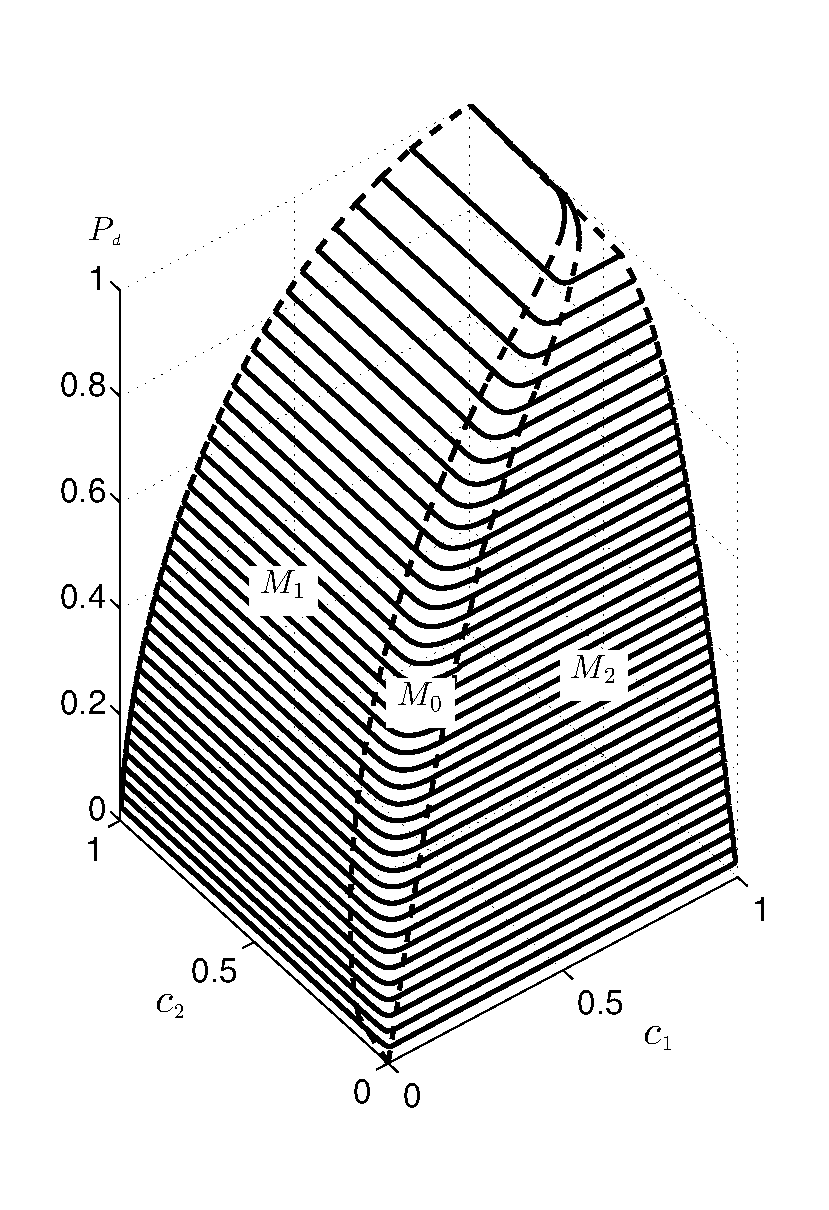
\includegraphics[width=12cm, height=16cm]{3/ROC2.eps}
\caption{The M-ROC surface for Gaussian Hypotheses.}
\label{pic: LJS}
\end{figure}

\noindent \textbf{Example 2:}

Next we consider a more general case of $M+1$ hypotheses given by 
\begin{equation}
\label{equ: m+1 Gaussian Hypo}
\begin{split}
H_0:\;\;\;\;\;\;&X\sim \mathcal{N}(\mu_0, \sigma_0^2)\\
H_1:\;\;\;\;\;\;&X\sim \mathcal{N}(\mu_1, \sigma_1^2)\\
  ......\\
H_M:\;\;\;\;\;\;&X\sim \mathcal{N}(\mu_M, \sigma_M^2)
\end{split}
\end{equation}
We will show when $\sigma_0^2 = \sigma_1^2 = ... = \sigma_M^2$ and $\mu_0 < \mu_i (i = 1, ..., M)$, the region achieved by ENP test with $k_i \geq 0 (i = 1, ..., M)$ degenerates to a curve.

Consider
\begin{equation}
\label{equ: define gx}
g(x) = \sum_{i=1}^{M}k_i\frac{f_i(x)}{f_0(x)}.
\end{equation}
Since 
\begin{equation}
\label{equ: gaussian PDF}
f_i(x) = \frac{1}{\sqrt{2\pi\sigma_i^2}}\exp(-\frac{(x-\mu_i)^2}{2\sigma_i^2}).
\end{equation}
we have
\begin{equation}
\label{g00}
g(x) = \sum_{i=1}^{M}k_i\frac{\frac{1}{\sqrt{2\pi\sigma_i^2}}\exp(-\frac{(x-\mu_i)^2}{2\sigma_i^2})}{\frac{1}{\sqrt{2\pi\sigma_0^2}}\exp(-\frac{(x-\mu_0)^2}{2\sigma_0^2})}
\end{equation}
Substitute  $\sigma_i^2 = \sigma_0^2 (i = 1, ..., M)$ into \eqref{g00}, we have 
\begin{equation}
\label{equ: gx cc}
g(x) = \sum_{i=1}^{M}k_i\exp(\frac{(\mu_i - \mu_0)(2x-\mu_i - \mu_0)}{2\sigma_0^2})
\end{equation}
Defining $p_i = \frac{\mu_i - \mu_0}{2\sigma_0^2}$, \eqref{equ: gx cc} can be written as
\begin{equation}
g(x) = \sum_{i=1}^{M}k_i\exp(p_i(2x-\mu_0 - \mu_i)
\end{equation}
From the condition $\mu_0 < \mu_i (i=1, ..., M)$, we can see $p_i >0$ and  $g(x)$ is a monotonically increasing function with $x$. Here from \textbf{Property 1} we know that $M_0$ (the region achieved by the ENP test with $k_i \geq 0 (i=1, ..., M)$) degenerates to a curve. Moreover, for a specific $\mathbf{c}$, the decision rule is 
\[
x \substack{H_0 \\ \leq \\ > \\ \bar{H}_0} x_0
\]
where $x_0 = \min\{F_1^{-1}(c_1), ..., F_M^{-1}(c_M)\}$. The associated probability of detection is
\[
P_d = F_0(x_0)
\]

Figure \ref{pic: surface for same variance} shows the M-ROC surface for $M=2$, $\mu_0 = 0$, $\mu_1 = 1$, $\mu_2 = 2$ and $\sigma_0^2 = \sigma_1^2 = \sigma_2^2 = 1$. The bold curve is region $M_0$. From the definition of $M_0$, we know $M_0$ is the region can also be achieved by both ENP test and the MENP test. We can see, comparing to the ENP test, the MENP test has a much larger achievable region (the MENP test can achieve the $P_d$ for the whole $c_1, c_2$ plane, while the ENP test can only achieve the $P_d$ when $c_1$, $c_2$ lies on region $N_0$, which is also a curve because $N_0$ is the projection of $M_0$). 

\begin{figure}[!t]
\centering
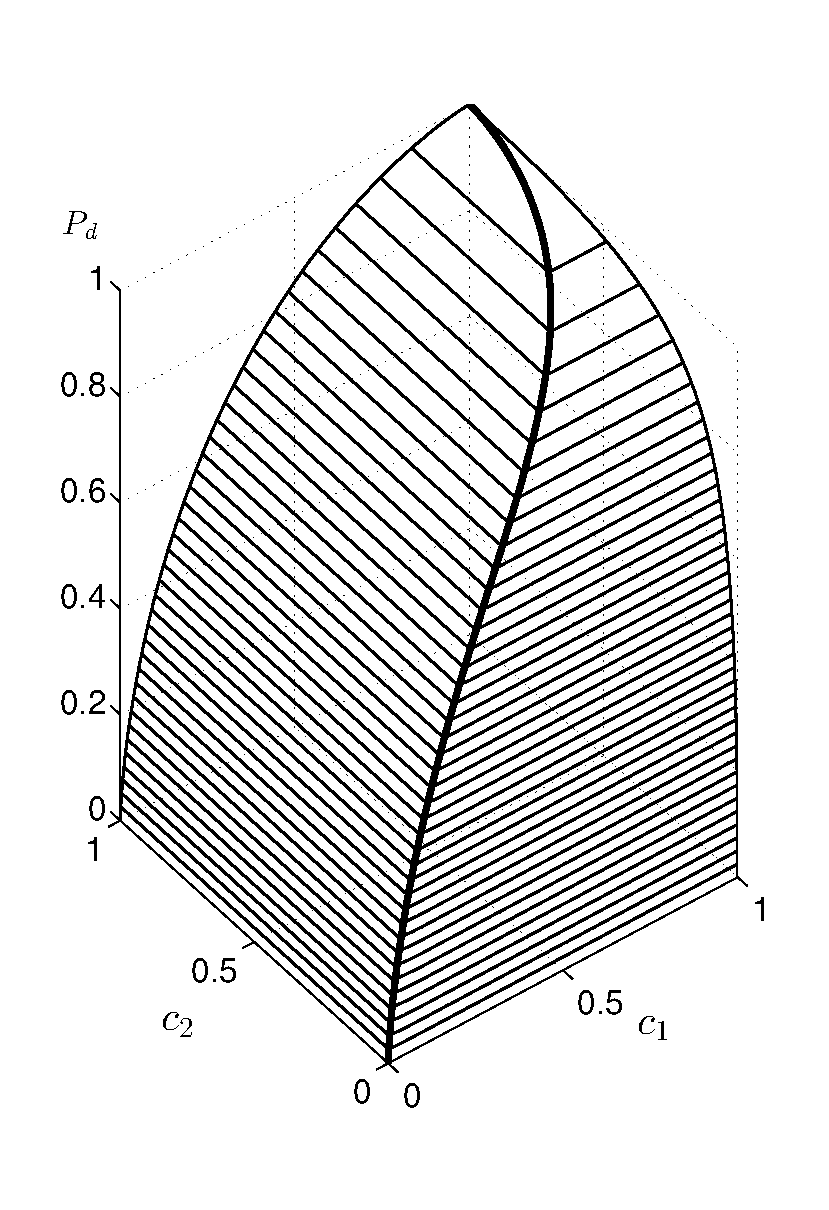
\includegraphics[width=12cm, height=16cm]{3/gaussian.eps}
\caption{The M-ROC for Gaussian distribution with same variance.}
\label{pic: surface for same variance}
\end{figure}
